\section{Introduction}
Coding theory expresses the mathematical view of point of codes used in error-correcting in communication theory. It has two branches; algebraic and combinatorial. This paper gives an introduction to algebraic coding theory. We start with linear codes over finite fields. As we mention rank-metric and Hamming-metric, our main focus will be on \textit{Hamming-metric}. Hamming-distance is connected to the error detection of a linear code by giving the number of changes we should do on a codeword to obtain another codeword. We give the general definitions of some important family of codes. Reed-Solomon codes, Reed-Muller codes, and Gabidulin codes are obtained by evaluations of polynomials, where the first two are defined on the Hamming-metric and the latter on rank-metric. We give the cyclic code definition to give a familiarity for permutation code equivalence for the later chapter, LDPC code definition just for general knowledge, and Goppa code definition as it is the first code family with an algebraic structure.\\
Our main objective is to give the reader a general introduction of algebraic coding theory to use this field in cryptography. We believe that this combination will be useful in modern problems, especially in preventing attacks on cryptosystems by quantum computers.  

\section{Algebraic Coding Theory}
\label{sec:algeb_coding}
Algebraic Coding Theory is concerned with developing, encoding, and decoding codes by using discrete mathematics. This section refers to all the fundamental definitions and coding-theoretic objects needed for code-based cryptography. 

\subsection{Basics on Hamming-Metric Codes}
Consider a finite field $\mathbb F_q$ of q elements where q is a prime power.
\begin{definition}[Linear Codes] Let $1 \leq k \leq n$ be positive integers. $C$ is an $[n, k]$ \textit{linear code} over $\mathbb F_q$, if $C$ is a $k$-dimensional linear subspace of $\mathbb F_q^n$.
\end{definition}

\noindent In other words, a \textit{code} is basically any subset $C \subseteq F_q^n$.
\\[0.4cm]
There are three main parameters. Then, the parameter $n$ is the \textit{length} and $k$ is the \textit{dimension} of the code $C$. Also, the other parameter $d_{\min}$ is the \textit{minimum distance} of the code $C$. In addition, elements of $C$ are called \textit{codewords}. 

For defining the minimum distance, firstly we give definition of Hamming Distance. 

\begin{definition}[Hamming Distance]
For $\textbf{x}, \textbf{y} \in \mathbb F_q^n$ the \textit{Hamming distance} between \textbf{x} and \textbf{y} is the number of components they differ with the same index and is given by
\[
\mathrm{d}_H(x, y) =
\left| \{\, i \in \{1, \dots, n\} 
\mid x_i \neq y_i \,\} \right|.
\]    
\end{definition}

\begin{definition}[Hamming Weight]
Let n be a positive integer. The \textit{Hamming weight} of 
$\textbf{x} \in \mathbb F_q^n$ is the number of non-zero components and is given by
\[
\mathrm{wt}_H(x) = 
\left| \{\, i \in \{1, \dots, n\} 
\mid x_i \neq 0 \,\} \right|.
\]
% \mathrm{...}
% \left| ... \right|
% \{ ... \}
% \mid -> such that
\end{definition}

\noindent Notice that for the linear codes, Hamming distance is an induced form of Hamming weight,
\[
\mathrm{d}_H(x, y) = \mathrm{wt}_H(x-y).
\]
as linear codes are closed under the operations of a finite field. In other words, we know that Hamming distance and Hamming weight are the same for linear codes.

\begin{definition}[Minimum Distance]
Let $C$ be a code over $\mathbb F_q$. The \textit{minimum Hamming distance} of $C$ is given by
\[
\mathrm{d}_H(C) = 
\min\{\,d_H(\textbf{x}, \textbf{y}) \mid 
\textbf{x}, \textbf{y} \in C, \textbf{x} \neq \textbf{y} \,\}.
\]
\end{definition}

The minimum distance between a vector $\mathbf{x} \in \mathbb{F}_q^n$ and a codeword $c \in C$ is denoted by $d_H(\mathbf{x}, C)$.\\[0.4cm]
For a positive integer $r$, we define \emph{Hamming ball} as all the vectors in $\mathbb{F}_q^n$ with Hamming weight at most $r$:
\[
B_H(r, n, q) =
\{\, \mathbf{x} \in \mathbb{F}_q^n \mid 
\mathrm{wt}_H(\textbf{x}) \leq \textit{r}\,\}.
\]
\\[0.4cm]
The minimum distance of a code is connected to the error correcting capacity of that code. A code can correct up to t errors if for all
$\mathbf{x} \in \mathbb{F}_q^n$ with $d_H(\mathbf{x}, C) \leq t$, there is a unique $\mathbf{y} \in C$ such that $d_H(\mathbf{x}, \mathbf{y}) \leq t$.\\[0.4cm]
We construct a \textit{decoding algorithm} $D$ to find the closest codeword $\mathbf{y} \in C$ such that $d_H(\mathbf{x}, \mathbf{y}) \leq t$ for a given
$\mathbf{x} \in \mathbb{F}_q^n$.\\[0.4cm]
\begin{proposition}
Let $C$ be a linear code over $\mathbb{F}_q^n$ with minimum distance $d_H$. $C$ can correct up to 
\[
t := \left\lfloor\frac{d_H - 1}{2}\right\rfloor.
\]
\end{proposition}

\begin{proof}
Set $2t\leq d_H-1$. Let $\mathbf{c_1}, \mathbf{c_2}\in C$ be distinct codewords. Then $d_H(\mathbf{c_1},\mathbf{c_2})\geq d_H$.\\
For a contradiction, say that there is a $\mathbf{y}$ such that
\[
\mathbf{y}\in B_H(\mathbf{c_1}, t) \cap B_H(\mathbf{c_2}, t).
\]
By the triangle inequality, we have
\[
d_H(\mathbf{c_1}, \mathbf{c_2})\leq d_H(\mathbf{c_1},\mathbf{y}) +d_H(\mathbf{c_1},\mathbf{y})\leq t+t=2t\leq d_H-1. 
\]
Then $d_H(\mathbf{c_1}, \mathbf{c_2})\leq d_H-1$, which contradicts the definition of Hamming distance. Thus, $B_H(\mathbf{c_1}, t)$ and $B_H(\mathbf{c_2}, t)$ are disjoint balls.\\[0.2cm]
Now let $y$ be any received word produced from $\mathbf{c}\in C$ with $d_H(y, \mathbf{c})\leq t$, that is, with at most $t$ errors. Then we know that $y\in B_H(\mathbf{c'}, t)$ if and only if $\mathbf{c'}=\mathbf{c}$. So, $c$ is the unique codeword of $y$ up to distance $t$. That is, $C$ can correct errors up to $t = \left\lfloor\frac{d_H - 1}{2}\right\rfloor$. 
\end{proof}

\begin{figure}[h]
    \centering
    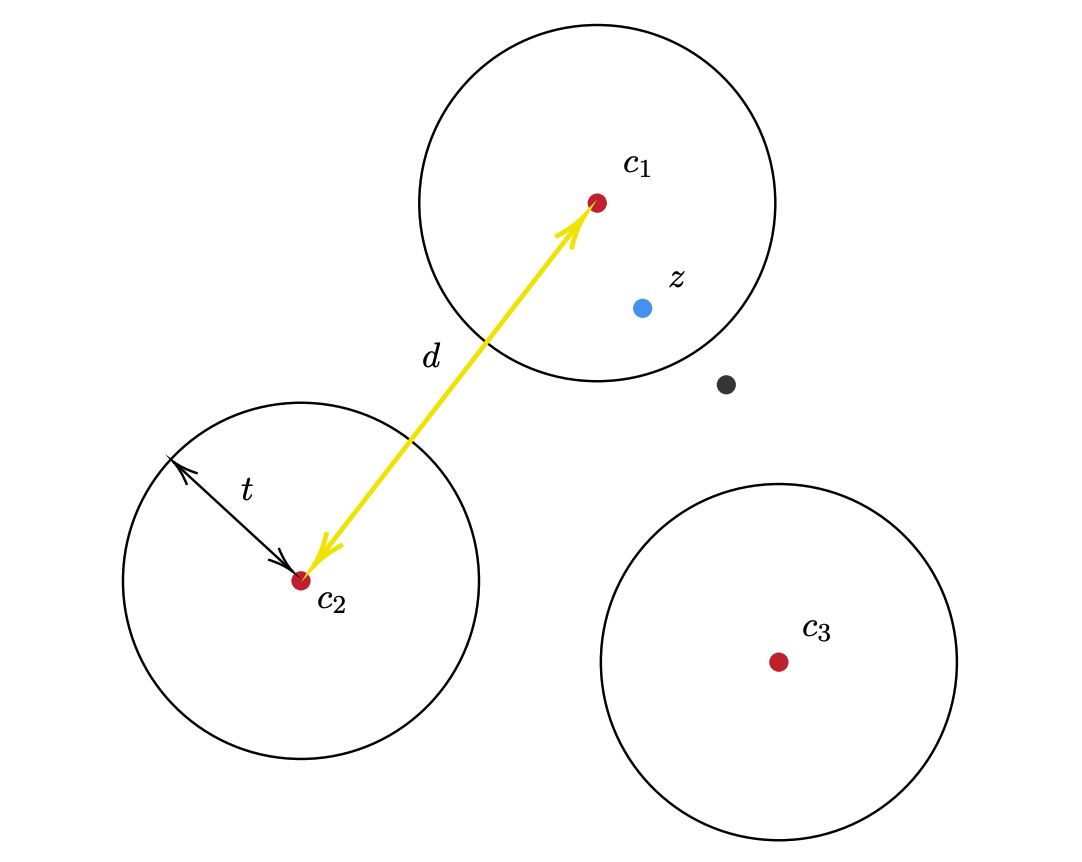
\includegraphics[scale=0.4]{balltheory.png}
    \caption{A visualization of the proof of \textbf{Proposition 1}.}
    \label{fig:ball}
\end{figure}
In this figure \ref{fig:ball}, we know that $c_1,c_2,c_3\in C$ are codewords and that the distance between each codeword is exactly $d$. And also if we have an error in the $z$ place, our code can correct it since the value of $t$.

\begin{theorem}[Singleton Bound]
\textit{Let $k \leq n$ be positive integers and $C$ an $[n, k]$ linear code over $\mathbb{F}_q$. Then,}
\[
d_H \leq n - k + 1.
\]
\end{theorem}

\begin{proof}
    Let $C$ be a linear code over $\mathbb{F}_q^n$ and define\\
    \begin{align*}
    \varphi&: C \xrightarrow{}\mathbb{F}_q^{n-d_H+1}\\
    &(c_1, c_2, \dots,c_n) \mapsto (c_1,c_2,\dots,c_{n-d_H+1}).\\   
    \end{align*} 
    Let $c,c' \in C$ and $\varphi(c)=\varphi(c')$.
    Then $d_H(c, c') \leq d_H-1$.
    But $d_H(C)=d_H$ so $d_H(c, c') \geq d_H$. So $c = c'$. 
    $\varphi$ is injective and $\varphi(C) \subseteq \mathbb{F}_q^{n-d_H+1}$. Then $q^{n-d_H+1}\geq|\varphi(C)|=|C|=q^k$.\\
    Thus, $d_H\leq n-k+1 $.
\end{proof}
We call the codes that achieve the Singleton bound \textit{maximum distance separable} (MDS) codes which can correct the maximum amount of errors.

\begin{definition}[Generator Matrix]
Let $k \leq n$ be positive integers and $C$ be an $[n, k]$ linear code over $\mathbb{F}_q$. Then, the matrix $\mathbf{G} \in \mathbb{F}_q^{k \times n}$ is \textit{generator matrix of} $C$ if 
\[
C = 
\{\, \mathbf{xG} \mid \mathbf{x} \in \mathbb{F}_q^k\,\},
\]
that is, the rows of $\mathbf{G}$ form a basis of $C$.
\end{definition}

\begin{definition}[Parity-Check Matrix]
Let $k \leq n$ be positive integers and $C$ an $[n, k]$ linear code over $\mathbb{F}_q$. Then, the matrix $\mathbf{H} \in \mathbb{F}_q^{(n-k) \times n}$ is \textit{parity-check matrix of} $C$ if
\[
C = 
\{\, \mathbf{y} \mid \mathbf{Hy}^T = 0\,\}.
\]
\end{definition}
Parity-check matrices are involved in error detection.
We call $\mathbf{xH}^T$ a \textit{syndrome} for any $\mathbf{x} \in \mathbb{F}_q^n$.

\begin{definition}[Dual Code]
Let $k \leq n$ be positive integers and $C$ an $[n, k]$ linear code over $\mathbb{F}_q$. $C^\perp$ $[n, n-k]$ linear code over $\mathbb{F}_q$ is the \textit{dual code} of $C$ defined as
\[
C^\perp =
\{\, \mathbf{x} \in \mathbb{F}_q^n \mid \langle \mathbf{x}, \mathbf{y} \rangle = 0 \quad \forall y \in C\,\}.
\]
\end{definition}

\begin{proposition}
A parity-check matrix $\mathbf{H}$ of $C$ is a generator matrix of $C^\perp$. 
\end{proposition}
\begin{proof}
    By the definition of parity-check matrix $H$, we have $\mathbf{c}H_i^T=0$ where $H_i$ is the $i^{th}$ row of $H$ for $\mathbf{c}\in C$. Then $H_i\in C^\perp$. Thus $rowspan(H) \subseteq C^\perp.$\\
    The duality gives $\dim(C)+\dim(C^\perp)=n$ so $\dim(C^\perp)=n-k$.\\
    As the syndrome of $C$ defines the error patterns, $H$ have independent rows, thus it has full row rank, that is, $\dim(rowspan(H))=n-k$.\\
    Then we have $\dim(C^\perp)=dim(rowspan(H))=n-k$. With the inclusion above, we can conclude that $rowspan(H) = C^\perp$.
    Therefore, rows of the parity-check matrix $H$ of $C$ form a basis for the dual code $C^\perp$.
\end{proof}
\vspace{1.0cm}
\begin{definition}[Information Set]
Let $k \leq n$ be positive integers and $C$ an $[n, k]$ linear code over $\mathbb{F}_q$. A set $I \subset \{\,1, \dots, n\,\}$ of size $k$ is an \textit{information set} of $C$ if
\[
\left|C_I\right| = \left|C|\right. 
\]
\end{definition}
\begin{exmp}
Let $C$ be the code generated by $G \in \mathbb{F}_5^{2 \times 4}$, given as
\[
\mathbf{G} =
\begin{pmatrix}
1 & 3 & 2 & 3 \\
0 & 4 & 4 & 3
\end{pmatrix}.
\]
Determine all information sets of this code.
\end{exmp}
\begin{solution}
    Information set of $C$ is $I \subset \{\,1,2,3,4\,\}$ of size $k=2$. We want the columns of $G$ that are linearly independent.\\

\begin{equation*}
    \det\begin{pmatrix}
        1&3\\0&4
    \end{pmatrix}=4\neq0, \quad
    \det\begin{pmatrix}
        1&2\\0&4
    \end{pmatrix}=4\neq0, \quad
    \det\begin{pmatrix}
        1&3\\0&3
    \end{pmatrix}=3\neq0,
\end{equation*}
\begin{equation*}
    \det\begin{pmatrix}
        3&2\\4&4
    \end{pmatrix}=4\neq0, \quad
    \det\begin{pmatrix}
        3&3\\4&3
    \end{pmatrix}=-3\neq0, \quad
    \det\begin{pmatrix}
        2&3\\4&3
    \end{pmatrix}=-6\neq0.
\end{equation*}
    
All matrices are invertible, thus all information sets of $C$ are $\{1,2\},\{1,3\},\{1,4\},\{2,3\},\{2,4\},\{3,4\}.$
\end{solution}

\subsection{Generalized Reed-Solomon Codes}
Now we can introduce the important codes used in code-based cryptography. The first code will be an error-correction code called Generalized Reed-Solomon codes (GRS). Reed-Solomon codes are the first codes we will see that are obtained by polynomial evaluation.

\begin{definition}[Reed-Solomon Codes]
Let $k \leq n \leq q$ be positive integers. Let $\alpha \in \mathbb{F}_q^n$ be an n-tuple of distinct elements and $\beta \in \mathbb{F}_q^n$ be an n-tuple of nonzero elements. The \textit{Generalized Reed-Solomon code} of length $n$ and dimension $k$ is defined as
\[
GRS_{n,k}(\alpha, \beta) = \{\, (\beta_1f(\alpha_1), \dots, \beta_nf(\alpha_n)) \mid f \in \mathbb{F}_q[x], deg(f) < k \,\}.
\]
\end{definition}

When $\beta = \{\,1, \dots,1 \,\}$, we define \textit{Reed-Solomon codes} as
\[
RS_{n,k}(\alpha) = \{\, (f(\alpha_1), \dots, f(\alpha_n)) \mid f \in \mathbb{F}_q[x], deg(f) < k \,\}.
\]

\begin{proposition}
The Vandermonde matrix 
\[
\begin{pmatrix}
1 & \dots & 1 \\
\alpha_1 & \dots & \alpha_n \\
\vdots && \vdots \\
\alpha_n^{k-1} & \dots & \alpha_n^{k-1}
\end{pmatrix}
\]
is a generator matrix of a RS codes.
\end{proposition}

\begin{proof}
    Define $G$ as the Vandermonde matrix.
    Let $c\in RS_{n,k}(\alpha,\beta)$ any codeword in the form of 
    \[
    c = (f(\alpha_1),\dots,f(\alpha_n))
    \]
    where $f\in \mathbb{F}_q[x]$ of degree less than $k$. Then $f(x) = a_0+a_1x+a_2x^2+\dots+a_{k-1}x^{k-1}$. So we have
    \[
    c = (a_0+a_1\alpha_1,\dots,a_{k-1}\alpha_1^{k-1}, a_0+a_1\alpha_2,\dots,a_{k-1}\alpha_2^{k-1}, \dots,
    a_0+a_1\alpha_n,\dots,a_{k-1}\alpha_n^{k-1}) =
    \]
    \[
    (a_0(1,\dots,1),a_1(\alpha_1,\dots,\alpha_n),\dots,a_n(\alpha_1^{k-1},\dots,\alpha_n^{k-1})).
    \]
    which gives a linear combination of rows of $G$. Thus, we can say that the rows of $G$ span $RS_{n,k}(\alpha,\beta)$.\\
    Now assume that
    \[
    a_0(1,\dots,1)+a_1(\alpha_1,\dots,\alpha_n)+\dots,a_n(\alpha_1^{k-1}+\dots+\alpha_n^{k-1} = 0
    \]
    which implies that
    \[
    a_0+a_1\alpha_i+\dots+a_{k-1}\alpha_i^{k-1} = 0
    \] for any $i = 0,1\dots,n$. Then $f(\alpha_i)=0$ for any $i\in \{1,\dots,n\}$. By the definition of Reed-Muller codes, $n\geq k$. So $f$ with degree $k-1$ having $n$ roots is possible only if $f(x)$ is a zero polynomial. That is $a_0=a_1=\dots=a_{k-1}=0$. Thus, the rows of $G$ are linearly independent.
\end{proof}

\subsection{Goppa Codes}
Another code family that belongs to error-correcting codes is \textit{q-ary Goppa codes}. Goppa codes are the first algebraic geometric codes. Binary Goppa codes are used in the introduction of the \textit{McEliece framework}. We are going to discuss the McEliece framework in the cryptography section.

Let $m$ be a positive integer and $q$ be an prime number. Let $n = q^m$ and $\mathbb{F}_{q^m}$ be a finite field. Let $G \in \mathbb{F}_{q^m}[x]$. Define the quotient ring as
\[
S_m = \mathbb{F}_{q^m}[x] / \langle G \rangle.
\]

\begin{definition}[Classical Goppa Codes]
Let $\alpha \in \mathbb{F}_{q^m}^n$ be an n-tuple of distinct elements and $G(\alpha_i) \neq 0$ for all $i \in \{\,1, \dots, n \,\}$. We define the \textit{classical q-ary Goppa codes} as
\[
\Gamma(\alpha, \beta) = 
\{\,c \in \mathbb{F}_q^n \mid \sum_{i = 1}^n \frac{c_i}{x - \alpha_i} = 0 \text{ in } S_m \,\}.
\]
\end{definition}

The parity-check matrix of a Goppa code is defined as
\[
\mathbf{H}=\begin{pmatrix}
    G^{-1}(\alpha_1)&\dots&G^{-1}(\alpha_n)\\
    G^{-1}(\alpha_1)\alpha_1&\dots&G^{-1}(\alpha_n)\alpha_n\\
    \vdots&&\vdots\\
    G^{-1}(\alpha_1)\alpha_1^{r-1}&\dots&G^{-1}(\alpha_n)\alpha_n^{r-1}\\
\end{pmatrix}
\]
which is just a weighed Vadermonde matrix. This gives a connection between the classical Goppa codes and the GRS codes. 
For this connection, we define \textit{subfield subcode} of an $[n,k]$ linear code $C$ as 
\[
C_{\mathbb{F}_q} = C \cap\mathbb{F}_q^n.
\]
The subfield subcode of $GRS$ codes are called \textit{alternant codes}. Take $\alpha\in \mathbb{F}_{q^m}^n$ pairwise distinct and $\beta\in(\mathbb{F}_{q^m}^\ast)^n$ and we can define as
\[
A_{m,n,k}[\alpha,\beta]=GRS_{m,n,k}[\alpha,\beta]\cap\mathbb{F}_q^n.
\]
Goppa codes are the alternant codes. Here, GRS codes are particularly chosen with the weights $\beta_i = g(\alpha_i)^{-1}$ for a Goppa polynomial $g$.\\[0.2cm] 

We will finish this section by giving an example of a binary Goppa code.
\begin{exmp}
    Choose parameters $[n, m, t]$ as $[3, 3, 2]$.\\
    Represent $\mathbb{F}_8 \cong \mathbb{F}_2[x]/ \langle x^3+x+1 \rangle$. Let $\alpha$ be the root of $x^3+x+1$. So \[\mathbb{F}_8 = \{\,0,1,\alpha,\alpha^2,\alpha+1,\alpha^2+\alpha, \alpha^2+\alpha+1,\alpha^2+1\,\}.\] 
    Let be the irreducible polynomial $G = x^2+x+1 \in \mathbb{F}_8[x]$.\\
    Construct the quotient ring $S_3 = \mathbb{F}_8/\langle x^2+z+1\rangle.$\\
    Choose a set that avoids the roots of $G$ in $S_3$. Let this set be 
    $G'=\{\,1, \alpha^2,\alpha^2+1\,\}$, then
    \[        
    \noindent G(1)=1\\,G(\alpha^2)=\alpha+1\\,
    G(\alpha^2+\alpha+1)=\alpha^2+1\\,G(\alpha^2+1)=\alpha+1.
    \]\\
    Parity-check equations over $\mathbb{F}_2$ gives,
\begin{center}
    $\begin{pmatrix}
    1/G(1) &1/G(\alpha^2)& 1/G(\alpha^2+1)\\
    1/G(1) &\alpha^2/G(\alpha^2)& \alpha^2+1/G(\alpha^2+1)
    \end{pmatrix} = \begin{pmatrix}
    1 & \alpha+1 & \alpha+1\\
    1 & 1 & 1
    \end{pmatrix}.$\\[0.4cm]
\end{center}
    Expanding to $\mathbb{F}_2$ using 3-bit column vector we get,
\begin{center}
    $H=\begin{pmatrix}
        1&1&1\\
        0&1&1\\
        0&0&0\\
        1&1&1\\
        0&0&0\\
        0&0&0
    \end{pmatrix}.$\\[0.4cm]
\end{center}
    Dimension $k = n-rank(H)=3-2=1$. Thus, these parameter choice gives a trivial code, \[\Gamma(\alpha, \beta) = \{\,(0,0,0)\,\}.\]
    One can choose a greater $n$ for a non-trivial Goppa code.
\end{exmp}


\subsection{Cyclic Codes}
Let $c=\{c_1, c_2, \dots, c_n\} \in \mathbb{F}_q^n$, then its \textit{cyclic shift} is denoted as
\[
\sigma(c) = \{c_n, c_1, \dots, c_{n-1}\}.
\]

\begin{definition}[Cyclic Codes]
An $[n, k]$ linear code $C$ over $\mathbb{F}_q$ is \textit{cyclic} if $\sigma(C) = C$. That is, all the cyclic shifts of $C$ are again in $C$.    
\end{definition}
We call $C$ a \textit{quasi-cyclic} (QC) code if there is $l \in \mathbb{N}$, such that $\sigma_l(C) = C$

\subsection{LDPC}
In this section, we introduce a code family with no algebraic structure called \textit{low-density parity-check} (LDPC) codes. First, we will define \textit{row-weight}, or respectively \textit{column-weight} of a matrix. If each row of a matrix has Hamming weight $w$, we say that the matrix has row-weight $w$, or column weight $w$ if each column has Hamming weight $w$ so the main idea of the LDPC codes are sparse parity-check matrices. The common definition used in cryptography of LDPC codes is as follows.

\begin{definition}
Let $w \in \mathbb{N}$ be constant. An $[n, k]$ linear code $C$ over $\mathbb{F}_2$ is called a $w$-\textit{LDPC} code, if $C$ has a parity-check matrix $\mathbf{H} \in\mathbb{F}_q^{(n-k)\times n}$ with row-weight $w$.
\end{definition}



\subsection{Reed-Muller Codes}

Reed-Muller codes are another code structure obtained from evaluation of polynomials. Reed-Muller codes use multivariate polynomials as opposed to Reed-Solomon codes, which use one variable polynomials.

Let $p$ be a prime, $m,r$ be positive integers, and $q = p^n$. Let $\mathbb{F}_q[x_1, \dots, x_m]_\leq r$ be the $\mathbb{F}_q$-vector space of polynomials with $m$ variables and degree at most $r$. Fix an order $\{\, \alpha_1, \dots, \alpha_{q^m} \,\}$ of $\mathbb{F}_q^m$.

\begin{definition}
The \textit{Reed-Muller} code $RM_q(m, r)$ over $\mathbb{F}_q$ is the image of the map
\[
ev:\mathbb{F}_q[x_1, \dots, x_m]_\leq r \xrightarrow{} \mathbb{F}_q^{q^m}
\]
where
\[
ev(f) = (f(\alpha_1), \dots, f(\alpha_{q^m})).
\]
\end{definition}

We can compute the dimension and minimum distance of the Reed-Muller codes for $q = 2$.

\begin{proposition}
Let $r \leq m$. Then $dim_{\mathbb{F}_2}(RM_2(m, r)) = 
\sum_{i=0}^r {m\choose i}$ and the minimum distance of $RM_2(m, r) = 2^{m-r}$.
\end{proposition}

In the literature, there are other codes that are Reed-Muller type of codes. For example, Generalized Reed-Muller codes, Projective Reed-Muller Codes, Weighted Projective Reed-Muller Codes, etc. In this project, we've also discussed the differences of these codes. In WPRM codes for a fixed degree, Reed-Muller type codes on weighted projective spaces consider other parameters as well, regarding the weights coming from the space. Thus, the behavior of these Reed-Muller type codes is not only determined by degree $r$. A more detailed explanation can be found in \cite{WPS2023, WPS2025, Proj}.

\subsection{Rank-Metric Codes}

Until this section, we have talked about the Hamming-metric. We can use other metric spaces in coding theory. In this section, we introduce rank-metric and consider this metric for codes.

\begin{definition}{Rank Metric}
The \textit{rank weight} of $\mathbf{x}\in \mathbb{F}_{q^m}^n$ is given by
\[
wt_R(\mathbf{x}) = dim_{\mathbb{F}_q}(\langle x_1,\dots,x_n\rangle).
\]

The \textit{rank distance} of $\mathbf{x},\mathbf{y}\in \mathbb{F}_{q^m}^n$ is given by
\[
d_R(\mathbf{x},\mathbf{y})=wt_R(\mathbf{x}-\mathbf{y}).
\]

The \textit{minimum rank distance} of a linear code $C\subseteq \mathbb{F}_{q^m}^n$ is given by
\[
d_R(C)=\min\{\,wt_R(\mathbf{c}\mid\mathbf{c}\neq0, \mathbf{c}\in C\,\}.
\]
Rank-metric codes are a more broad subject, but for this paper only the general definitions will be enough.    
\end{definition}

\subsection{Gabidulin Codes}
Another evaluation code we will see are the Gabidulin codes. There are the first rank-metric code used in code-based cryptography.

Let $P_l$ be the $q$-polynomials of $q$-degree up to $l$ over $F_{q^m}$ so that
\[
P_l = \{\, \sum_{i=0}^df_ix^{q^i} \mid d \leq l \,\}.
\]

The definition is similar to that of Reed-Solomon codes.

\begin{definition}[Classical Gabidulin Codes]
Let $k \leq n \leq m$ be positive integers and $g \in \mathbb{F}_{q^m}^n$ have independent components. The \textit{classical Gabidulin} code $C$ over $\mathbb{F}_{q^m}^n$ of dimension $k$ is
\[
C = 
\{\, (f(g_1), \dots, f(g_n)) \mid f \in P_{k-1} \, \}.
\]
\end{definition}
Before giving the definition of generalized Gabidulin codes, we define the rank analog of the Vandermonde matrix.

\begin{definition}[Moore Matrix]
Let $v \in \mathbb{F}_{q^m}^n$ have $\mathbb{F}_q$-linearly independent components. The \textit{s-Moore matrix} is
\[
M_{s, k}(v_1, \dots, v_n) = 
\begin{pmatrix}
    v_1 &\dots& v_n \\
    v_1^{[s]} &\dots& v_n^{[s]} \\
    \vdots && \vdots \\
    v_1^{[s(k-1)]} &\dots& v_n^{[s(k-1)]} \\
\end{pmatrix} \in \mathbb{F}_{q^m}^{k \times n},
\]
where $[i] = q^i$.
\end{definition}

\begin{definition}[Generalized Gabidulin Codes]
Let $k \leq n \leq m$ be positive integers and $g \in \mathbb{F}_{q^m}^n$ have independent components and let $s$ and $m$  be positive integers with $gcd(s, m) = 1$. The \textit{generalized Gabidulin} code $C \subset \mathbb{F}_{q^m}^n$ of dimension $k$ is the row span of $M_{1, k}(g_1, \dots, g_n)$.    
\end{definition}

Thus, a generalized Gabidulin code is the rank analog of a generalized Reed-Solomon code.

\subsection{Code Equivalence}

\begin{definition}[Isometry]
Let $V$ be a space with distance map $d$. Linear map $\varphi: V \xrightarrow{}V$ is an \textit{isometry} if for all $\mathbf{x}, \mathbf{y} \in V$ we have $d(\mathbf{x}, \mathbf{y}) = d(\varphi(\mathbf{x}), \varphi(\mathbf{y}))$.    
\end{definition}

\begin{definition}[Code Equivalence]
Let $C_1, C_2 \subseteq V$ be linear codes. $C_1$ is \textit{equivalent} to $C_2$ if there is an isometry $\varphi \in I_d$ such that $\varphi(C_1) = \varphi(C_2)$.    
\end{definition}

\begin{definition}[Permutation Equivalence]
Code $C_1$ is \textit{permutation equivalent} to $C_2$ if there exists $\sigma \in S_n$ with $\sigma(C_1) = C_2$.    
\end{definition}

\begin{definition}[Linear Equivalence]
Code $C_1$ is \textit{linear equivalent} to $C_2$ if there exists an isometry $\varphi\in (\mathbb{F}_q^*)^n \rtimes S_n$ with $\varphi(C_1) = C_2$.  
\end{definition}

Permutation equivalent codes are also linear equivalent codes by definition.

\begin{proposition}
Let $C_1, C_2 \subseteq \mathbb{F}_q^n$ be permutation equivalent. Then for any generator matrix $\mathbf{G_1}$ of $C_1$ and $\mathbf{G_2}$ of $C_2$, there exists a $n \times n$ permutation matrix $\mathbf{G_1}$ and an invertible matrix $\mathbf{S} \in GL_k(q)$ such that
\[
\mathbf{SG_1P} = \mathbf{G_2}.
\]
If $C_1$ and $C_2$ are linear equivalent codes, then there is also a diagonal matrix $diag(\mathbf{v})$ for $\mathbf{v} \in (\mathbb{F}_q^*)^n$ such that
\[
\mathbf{SG_1P}diag(\mathbf{v}) = \mathbf{G_2}.
\]
\end{proposition}

\begin{proof}
    Let $C_1$ and $C_2$ be permutation equivalent. Then $\sigma(C_1) = C_2$ for some $\sigma\in S_n$.\\Let $G_1$ be the generator matrix of $C_1$ so that we have $C_2 = \{\mathbf{x}G_1P \mid\mathbf{x}\in \mathbf{F}_n^k\}$ where $P$ is a permutation matrix of $\sigma$. Thus, $G_1P$ is a generator matrix of $G_2$\\ We can obtain a generator matrix of $G_2$ of $C_2$ by using a different basis for $G_1P$. Thus we can find an invertible matrix $S \in GL_k{\mathbb({F}_q)}$ such that $G_2 = S(G_1P)$.\\
    A similar logic also applies for the second part.
\end{proof}

\begin{definition}[Rank-metric Equivalence]
Let $C_1, C_2 \subseteq \mathbb{F}_q^{m \times n}$. $C_1$ and $C_2$ are equivalent is there is an isometry $\varphi\in GL_m(q) \rtimes GL_n(q)$ such that $\varphi(C_1) = C_2$.
\end{definition}

\section{Conclusion}
Until now, we have seen the fundamental definitions and intuitions of algebraic coding theory. We mostly focused on Hamming-metric and only mention rank-metric. As this paper aims at constructing a basis for code-based cryptography, the reader can now continue with more broad types of code families, decoding algorithms, algebraic applications, and of course cryptography.